%TC:ignore
\documentclass[a4paper,12pt]{article}
\usepackage[english]{babel}
\usepackage{graphicx,wrapfig,lipsum}
\usepackage[svgnames, dvipsnames]{xcolor}
\usepackage{geometry}
\usepackage{caption} \captionsetup[figure]{font=footnotesize} % Ensure caption is loaded
\usepackage{subcaption} % For subfigure environment
\usepackage[comma,authoryear,round]{natbib}
\usepackage{amsmath} 
\usepackage{float}

\graphicspath{./images/}
\geometry{margin=1in, right=1.2in}
\linespread{1.3}

\hypersetup{
    pdftitle={Sharelatex Example},
    bookmarks=true,
    pdfpagemode=FullScreen,
}
\newcommand{\mpp}{MPP}
\newcommand{\hto}{H.T. Odum}


%TC:endignore

\begin{document}

\section[Intro]{Introduction to \mpp}

The restoration of fish migration in rivers has been recognized as a globally significant factor \citep{cox_fish_2023, cox_fish_2023a}. The present project considers these impacts. \textbf{This is bold.} And this is \textit{italic and \textbf{nested bold}}. \hto{} is important.

\subsection{A Sub-section}
Some text in a subsection. \texttt{Monospace text here}.

\begin{quotation}
    ``The Mismanagement of Power cannot be better shown, than by comparing the Effect of the Engine at Marly, with the Effects of the Water-works at London-Bridge.'' 
    \citep[p.~530]{desaguliers_course_1734}
\end{quotation}

\begin{figure}[H]
    \centering
    \begin{subfigure}{.48\textwidth} 
        \centering
        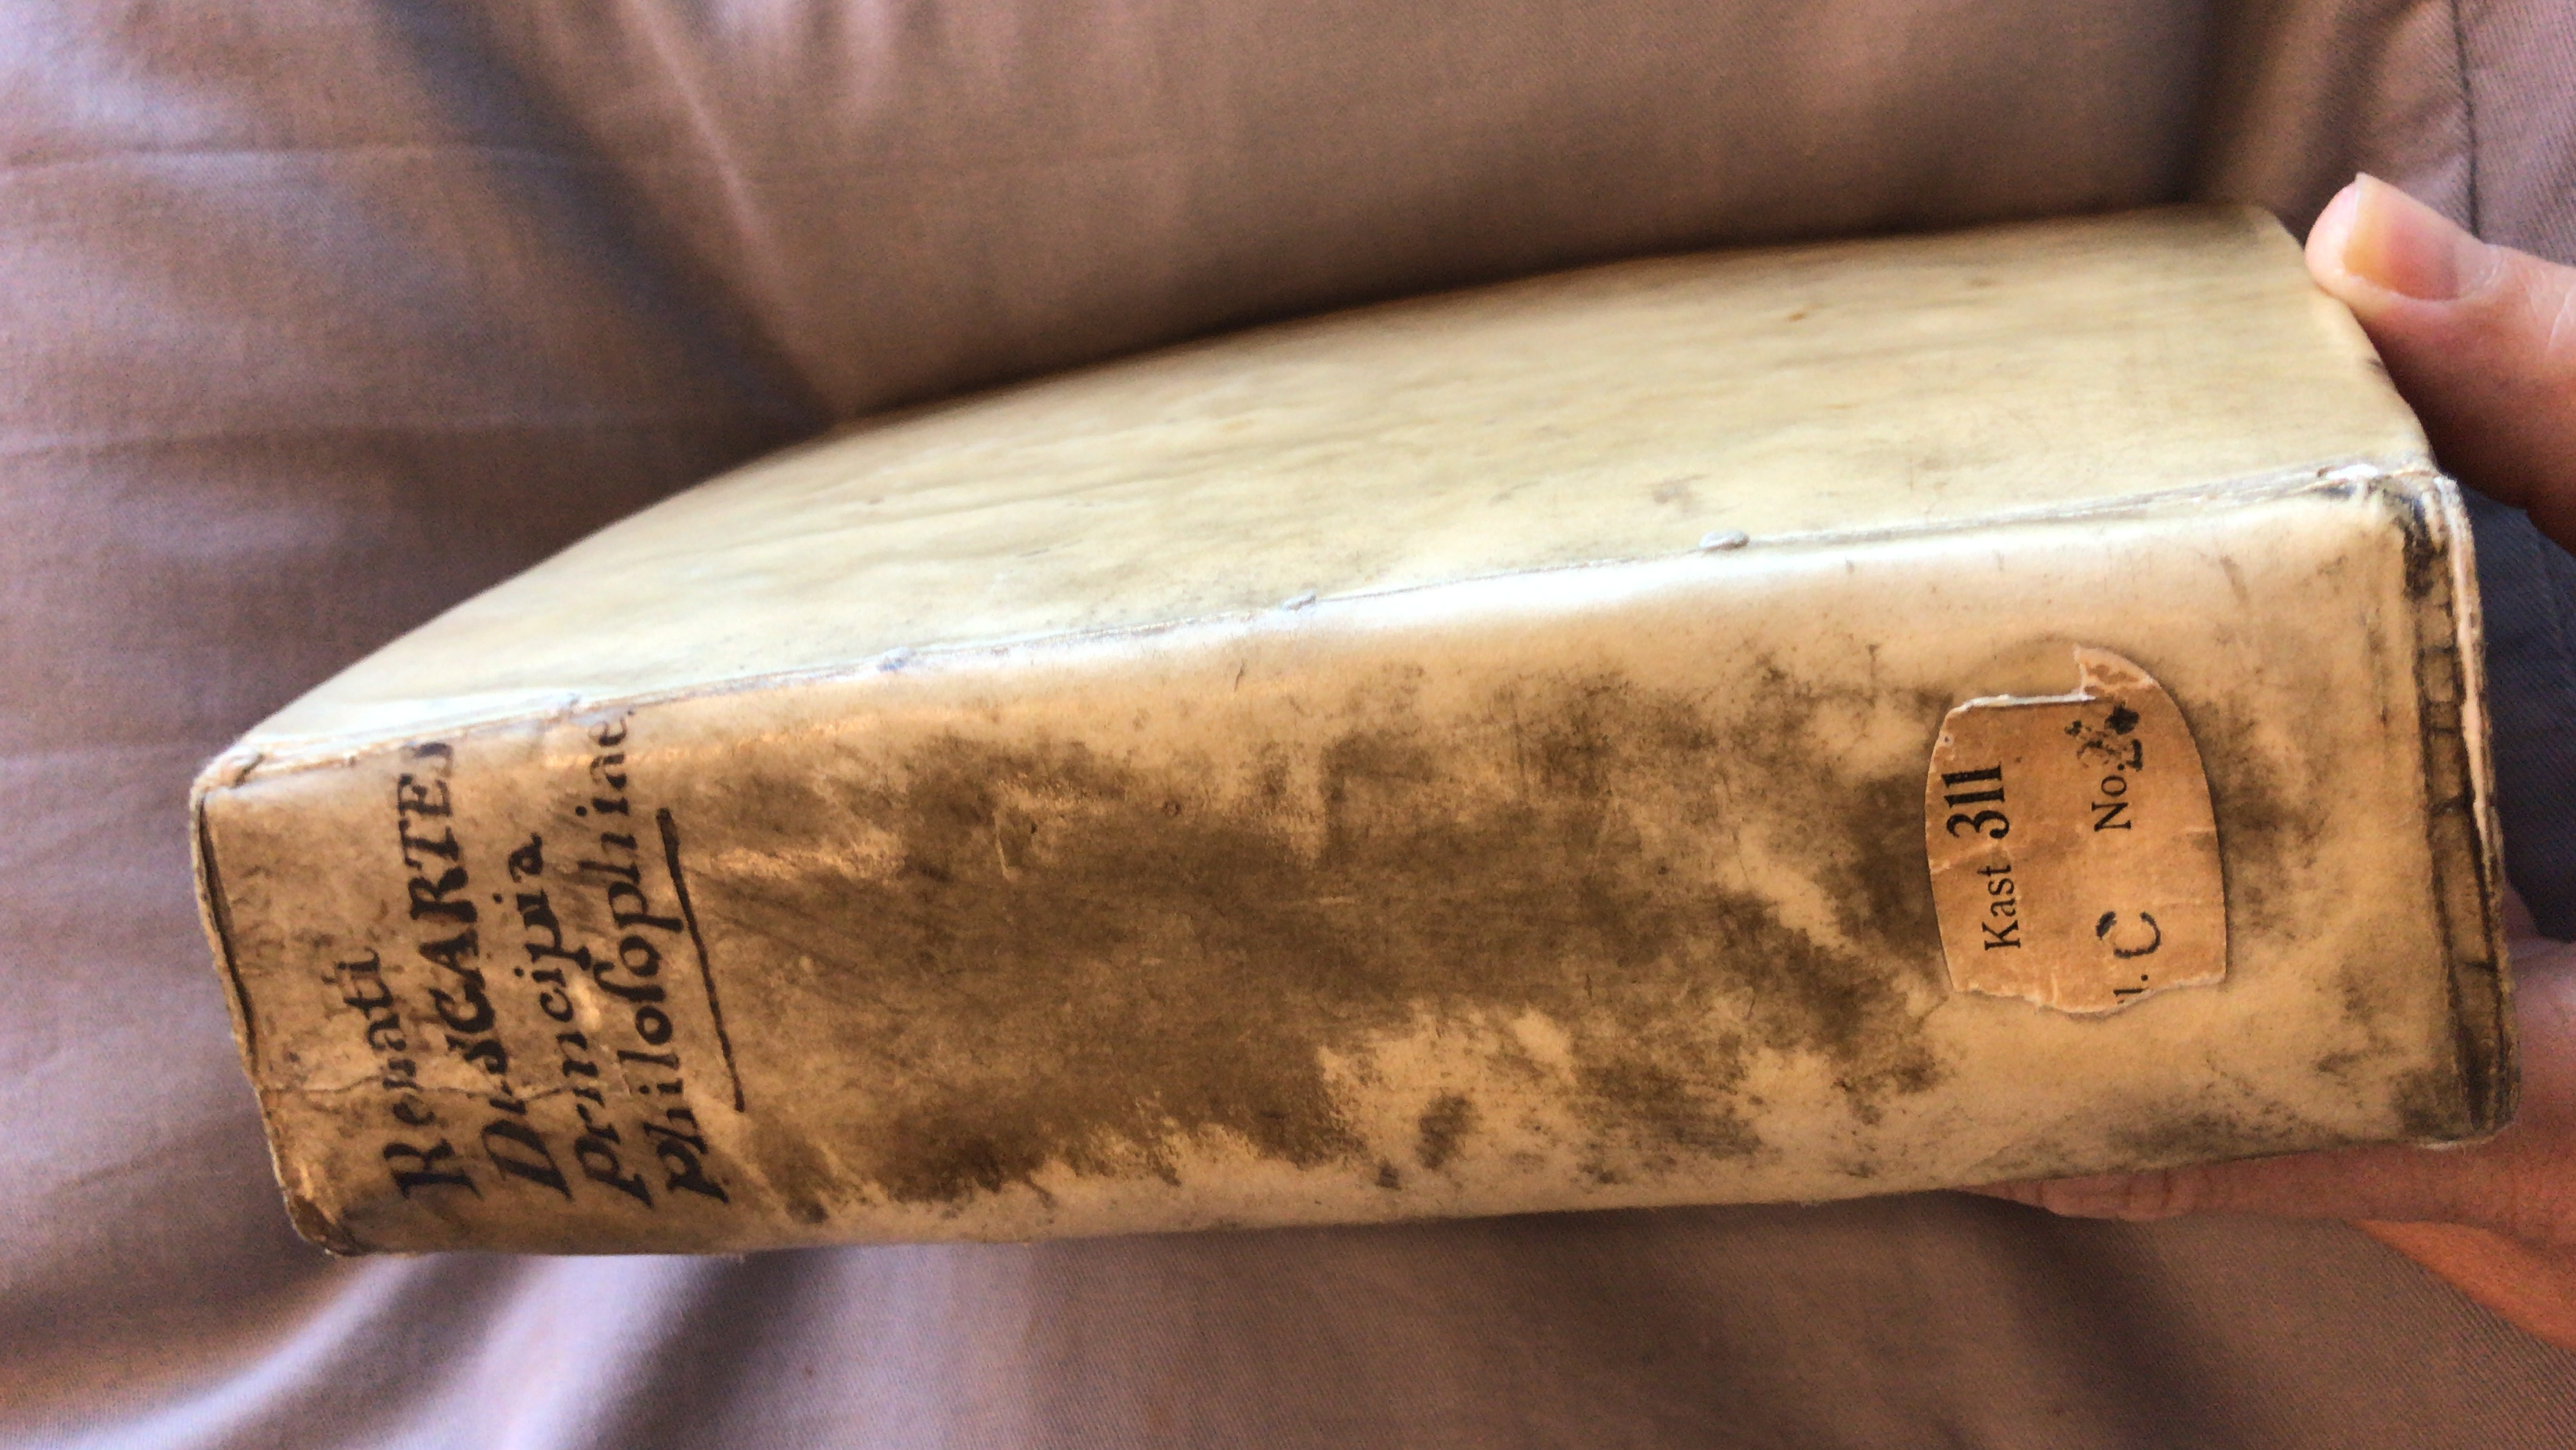
\includegraphics[width=.89\linewidth]{test.JPG}
        \caption{Subfigure caption: The water wheel design case by \citet[p.~101]{vitruvius_architectura_1511}}
        \label{fig:vitruvius}
    \end{subfigure}
    \caption{Overall figure caption for `\textit{Noria}' water wheel design using \mpp}
    \label{fig:waterwheel:contrast}
\end{figure}

An example list:
\begin{itemize}
    \item First item with \textbf{bold} part.
    \item Second item.
    \item \hto's principle, the \mpp.
\end{itemize}

A simple table:
\begin{tabular}{|l|c|r|}
\hline
Left & \textbf{Center} & Right \\
\hline
1 & 2 & 3 \\
data & more \textit{data} & final data \\
\hline
\end{tabular}

\newpage

Some more text after a page break. \url{https://example.com}

\bibliography{MyLibrary.bib}

\end{document}
    